\documentclass[conference]{IEEEtran}
%\IEEEoverridecommandlockouts
% The preceding line is only needed to identify funding in the first footnote. If that is unneeded, please comment it out.
\usepackage{cite}
\usepackage{amsmath,amssymb,amsfonts}
\usepackage{amsmath}
\usepackage{algpseudocode}
\usepackage{algorithm}
\usepackage{graphicx}
\usepackage{textcomp}
\usepackage{xcolor}
\usepackage{hyperref}
\def\BibTeX{{\rm B\kern-.05em{\sc i\kern-.025em b}\kern-.08em
    T\kern-.1667em\lower.7ex\hbox{E}\kern-.125emX}}
\begin{document}

\title{Parallel K-Means Clustering\\
{\footnotesize A parallel implementation of Hamerly's algorithm using OpenMP and MPI in C++}
}

\author{\IEEEauthorblockN{Filippo Pellizzari}
\IEEEauthorblockA{\textit{University of Trento} \\
\textit{Parallel programming course}\\
filippo.pellizzari@studenti.unitn.it (237822)}
}

\maketitle

\begin{abstract}
In this report, two k-means algorithms (Lloyd and Hamerly) are compared. Moreover, for Hamerly's version, a parallel implementation is presented and tested, using both a distributed memory (MPI) and a shared memory (OpenMP) framework in C++, to see the speedup over the standard case scaling with respect the number of points (N), the number of centroids (K) and the data dimensionality (D). Introducing a balancing strategy for the parallel execution.
\end{abstract}

\section{Introduction}
A clustering algorithm is an algorithm designed with the purpose of grouping, into an arbitrary number of classes, a set of points. Such classes are created by grouping together those points that have common features. Thus, the goal of this category of algorithms is to build knowledge about the data provided as input that makes it possible to find hidden relationships among them which can be used to classify a point whose class is not known a priori.

\section{Classical (or Lloyd) algorithm}

\subsection{Pseudocode}
The following pseudocode describes the basic implementation (lloyd algorithm) for the k-means clustering.

\begin{algorithm}[H]
  \caption{Lloyd algorithm}
  \begin{algorithmic}
    \State Repeat untill converge

    \For {each point}
      \State Calculate distance from every centroid
      \State Assign the point to the nearest centroid
    \EndFor 

    \For {each centroid}
      \State Calculate the new centroid by taking the mean of all points assigned to it
    \EndFor 
  \end{algorithmic}
\end{algorithm}

In this project, the distance is meant as Euclidean distance.

The convergence criterion could be the point when the centroids don't move more than a certain threshold or, as it is used in this project, after a fixed number of iterations.

\subsection{Tracking points during assignment}
The first, rather small, improvement with respect to the classical algorithm can be done during the point assignment to the closest centroid. In this project, two arrays have been introduced: the first one to track the number of points belonging to a certain class and the second one to store the sum of all coordinates of the points in every class (this latter has a dimension of $K \cdot D$). In this way, during the centroids update it is not necessary to iterate through all the points as the values needed to compute the average are already present inside the two arrays. Below is the pseudocode on how the point tracking has been handled in this project.

\begin{algorithm}[H]
    \caption{Point tracking}
    \begin{algorithmic}
      \State After the closest centroid has been found
      \If{Closest centroid is different from the old closest one}
        \State Decrement number of points in previous class and increment the new by one
        \State Remove coordinates from old class and add them to the new one
      \EndIf
    \end{algorithmic}
  \end{algorithm}
  
\section{Hamerly's Algorithm}
\subsection{Triangle inequality}
Hamerly's algorithm\cite{b1} is an optimization of the standard algorithm and exploits the fact that it is not necessary to recalculate the distance of each point from the centroids each time the latter are repositioned. Using the triangle inequality it is, in fact, possible to identify some points as criticals. Only for those points it is necessary to recalculate the closest centroid, while for the others, the previously assigned centroid is still the closest one.
The triangle inequality states that given 3 points A, B, C $\in \mathbb{R}^N$ then  
\begin{equation}
    \label{eq:triineq}
    |d(A, C) - d(B, C)| \leq d(A, B) \leq d(A, C) + d(B, C)
\end{equation}
    
\subsection{Upper and lower bound}
When a point is assigned to a new class, it tracks the distance from the closest centroid (upper bound, ub) and the distance from the second closest one (lower bound, lb). At this point, every time the centroids are updated, the lower and upper bounds of every point have to be updated as in the following pseudocode.

\begin{algorithm}[H]
    \caption{upper and lower bound update}
    \begin{algorithmic}
    \State ub += distance moved by point.centroid
    \If{points.centroid == centroid which moved the most }
        \State lb -= second max distance moved by a centroid
    \Else
        \State lb -= max distance moved by a centroid
    \EndIf
    \end{algorithmic}
\end{algorithm}

These updates are justified by Eq. (\ref{eq:triineq}) because, after the centroids have moved, the point won't by any farther than ub from its centroid and won't be any closer than lb to the second closest one. In this way, critical points are the ones for which $upper\_bound > lower\_bound$

\subsection{Time complexity}
In the case of Hamerly's algorithm, time complexity required to complete the classification is:
\begin{equation}
    D\cdot K\cdot N + mD(\phi N\cdot K + (1 - \phi)N)
    \label{eq:hamcomp}
\end{equation}
Where m is the number of iterations and $\phi$ is the percentage of critical points with respect to the total number of points.
The improvement over the standard algorithm lies in the fact that only the first time it is necessary to compute all the distances, whereas in subsequent iterations, for most points, there is no need to recompute the nearest centroid.

\section{Parallel Hamerly (OMP)}
Hamerly's algorithm can highly exploit parallelization to improve its performance. Indeed, when calculating the closest centroid for each point or when updating the centroids, it is possible to partition the points (in the first case) or the centroids (in the second case) between the threads to parallelize the calculations.
This is true at least for the first iteration. However, from the second one onward, partitioning the points is not as trivial because only for critical points need to be calculated the closest centroid. Because of this, simply splitting the points could lead one thread to have more criticals than another one.

\subsection{Partitioning points between the threads (1st iteration)}
If there are a total of T threads, the number of points that each thread will access is: $n = Int(N / T)$
Where Int(x) is the integer part of x. Moreover if the thread\_id is lower than $N\hspace{0.05in} mod\hspace{0.05in} T$ the number of points must be incremented by one. While iterating through the points, the access pattern will be $p = points[ thread\_id * n + off + j]$ where $off = N\hspace{0.05in} mod\hspace{0.05in} T$ if $thread\_id \geq N\hspace{0.05in} mod\hspace{0.05in} T $ , or $off = 0$ otherwise. 

\subsection{Load balancing}

After the centroids are updated, Hamerly's algorithm goes through all the points to update their lower and upper bounds. The load balancing strategy can be implemented during this phase as described by the following pseudocode.

After the balancing strategy, from the second iteration onward, the critials array can be partitioned between the threads, therefore giving each one the same workload.

\begin{algorithm}[H]
    \caption{Balancing strategy}
    \begin{algorithmic}
        \State \Comment In parallel
        \For{each point assigned to the thread}
        \State bounds update
        \If {ub $>$ lb}
            \State Add the point the local critical list
        \EndIf 
        \EndFor
        \State \Comment Sequentially
        \State create array that will contain all the criticals found
        \State \Comment In parallel
        \For{each critical found in thread}
        \State add it to the global array
    \EndFor
    \end{algorithmic}
\end{algorithm}

\section{MPI Version}
In the MPI version of the parallel Hamerly's algorithm, the idea is still the same used in the OMP version, i.e. for the first iteration, split the points between the threads and from the second one onward, partition the criticals found using the balancing strategy. For the centroids update just partition them between the processes. 

But, since every process has its own local storage and cannot access other's memory, the points and centroids partitioning and the communication during the load balancing phase needs to be handled using messages. 

\subsection{The main process}
In this implementation, process zero is the main process and contains all the information, i.e. the array with all the points, the array with all the criticals found in the last iteration, the centroids, the array with the number of points per class and the array with the sum of all coordinates per class. Regarding the centroids, each process has also its own copy of the full array because when calculating the class of a point, the process needs to compute all the distances.

\subsection{Scattering the data}
In the beginning of each phase (points or criticals assignment, centroids update and bounds update), process zero will scatter the needed items between the processes filling a local array where each process store the assigned ones. The needed items could be points or any other value that is needed to complete the phase, such as the array with the points per class and the average of all points array, for the centroids update. At the end of the work, process zero will gather the items back and update its memory by accounting for the gathered and updated values. In the case of the centroids update, after that process zero has gathered the updated ones, it will broadcast the full centroids array to all other processes to keep their memory updated. Another value that must be shared across all processes is the number of criticals found during the last iteration because it is needed by each process when calculating the number of points it has to access during the critical assignation.

\begin{figure*}
    \centering
    \caption{Speedups results}
    \label{fig:test_res}
    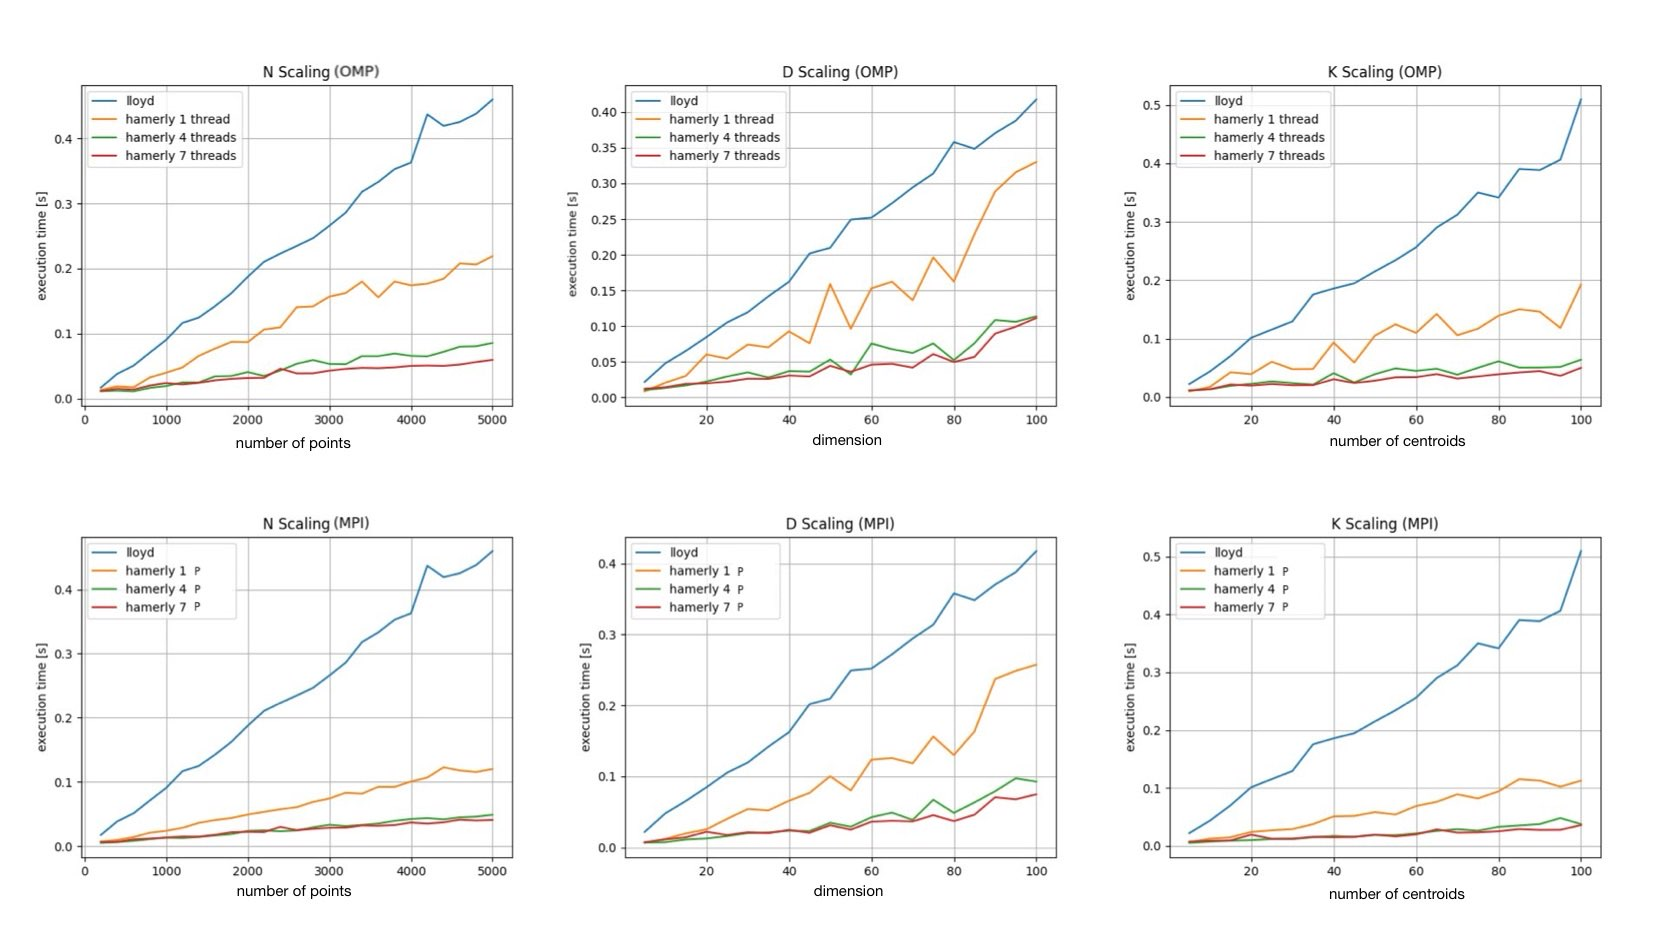
\includegraphics[width = 0.8\textwidth]{imgs/times.jpg}
\end{figure*}
\section{Testing}
\subsection{Scaling over N, K, D}
To test how the algorithm scales over the main dimensions a random dataset has been generated for each test (N scaling, K scaling and D scaling). This allows scaling over any dimension without breaking the logic of the dataset (since it is random). 

The dimension of the random datasets have been chosen to keep the product $N\cdot K\cdot D$ constant and equal to 200000. Depending on the scaling, the associated dimension should be large enough to allow an appropriate sweep. 

In specific, the dimensions used are (5000, 10, 4) for the N scaling, (500, 100, 4) for the K scaling and (500, 4, 100) for the D scaling. The constant 200000 have been chosen to keep a relatively high workload but still not too big to keep the execution times small. Section \ref{sec:diff_loads} describes what happens when changing that constant.

For every scaling test, the lloyd algorithm has been executed to fix a reference time. After that, the OMP and the MPI version have been executed with 1 to 10 threads (or processes). Every algorithm ran for a total of 20 iteration and is executed for 5 times to average the time results. The process has been repeated each time increasing the tested dimension. The results of these tests are shown in Figure \ref{fig:test_res} where the first line represent the OMP testing while in the second line are the MPI plots.

As expected the result is a straight line pattern because, no matter which dimension is scaling, Equation \ref{eq:hamcomp} can be reduced to one of the type y = mx + q.

\subsection{Speedups}
Even with one thread, Hamerly's algorithm shows a significant improvement in the execution time. However, increasing the number of threads results in even better performances as shown in the plots of Figure \ref{fig:su_res}. To calculate the speedups has been used the following formula
\begin{equation}
  su = 1 - Hamerly\_time / lloyd\_time
\end{equation}

\section{Testing with different workloads\label{sec:diff_loads}}
\subsection{workload too low}
If the total complexity of the dataset ($N\cdot K\cdot D$) is too low, then increasing the level of parallelism is no longer an improvement because the overhead needed to handle the parallel execution become too large with respect to the overall load and slow down the execution. This behavior has been tested using a real dataset\footnote{https://archive.ics.uci.edu/dataset/52/ionosphere} where the goal is to classify, as either bad or good, signals coming from the ionosphere testing the number of free electrons in the latter. The total complexity of the dataset is $N\cdot K\cdot D = 351 \cdot 2\cdot 34 = 23.869$ which is well below the tested load of 200000.

The speedup graph shows that increasing the number of threads reduces the speedup and therefore the execution times are higher when the number of threads is greater.
\centerline{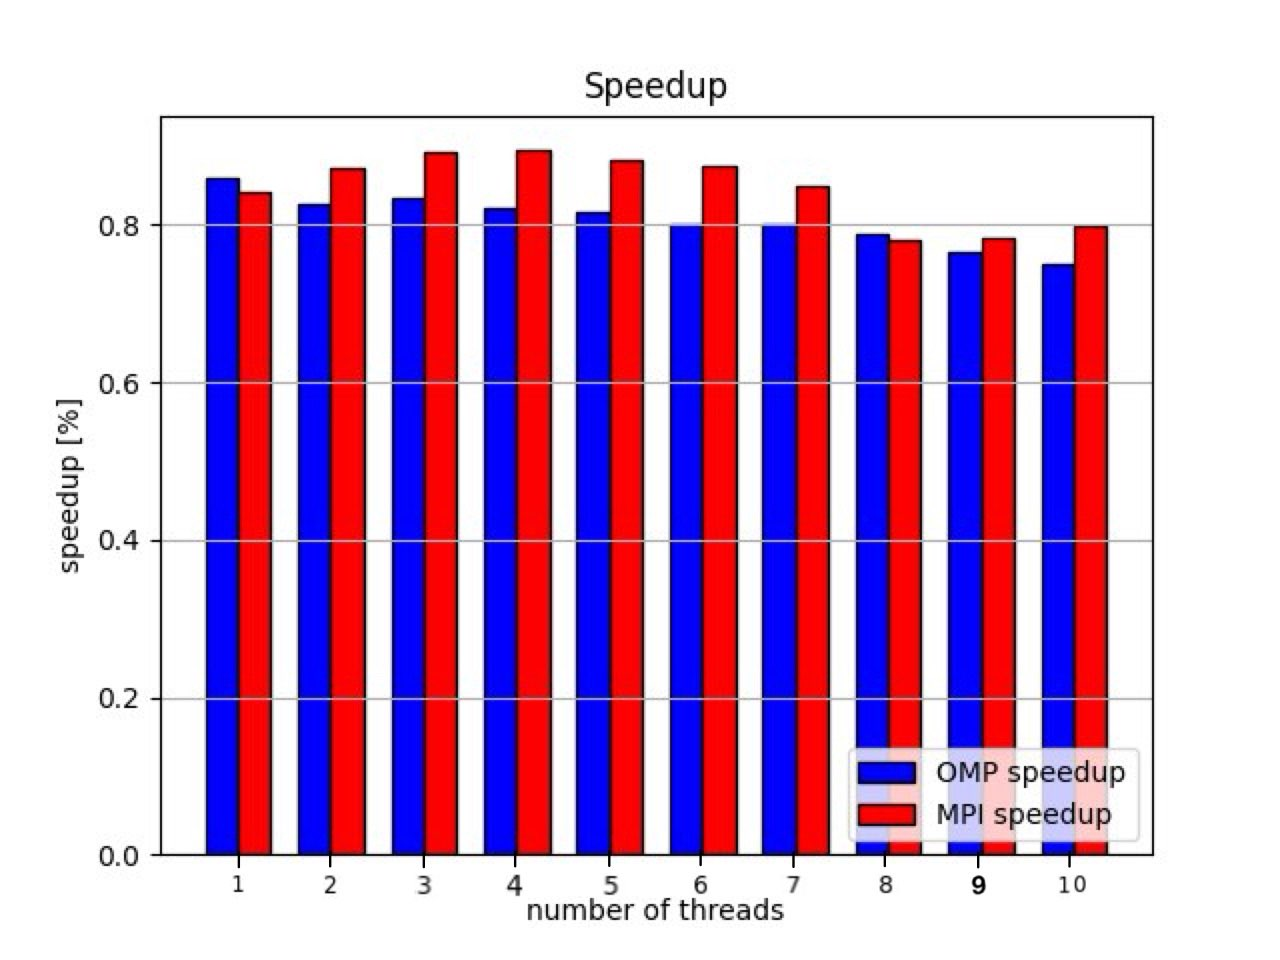
\includegraphics[width = 0.3\textwidth]{imgs/suiono.jpg}}

\begin{figure*}
  \centering
  \caption{OMP vs MPI speedup on medium complexity dataset}
  \label{fig:su_res}
  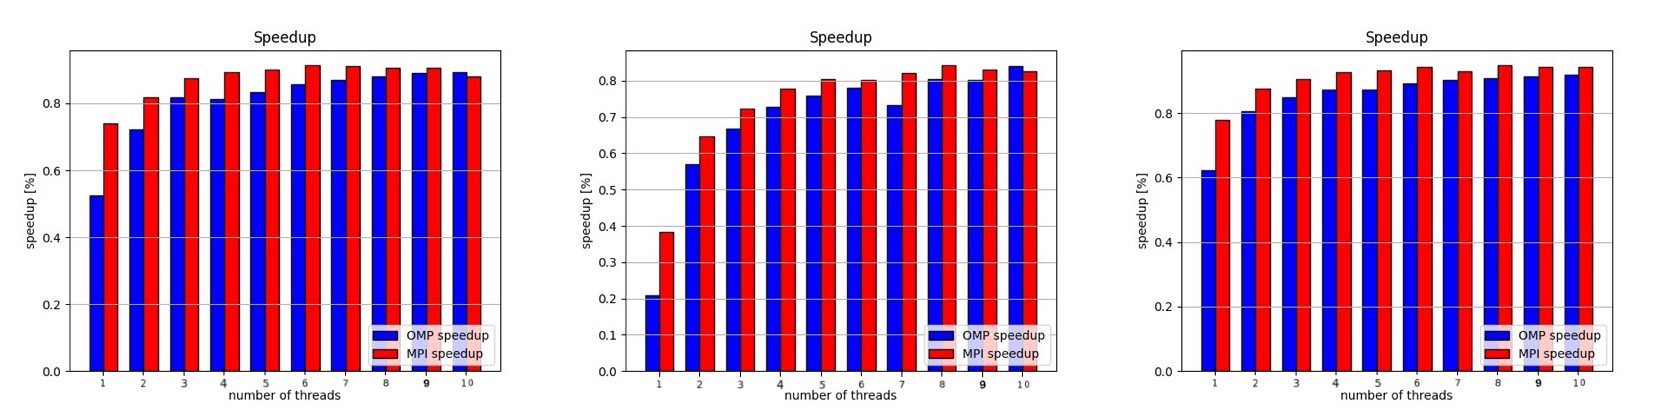
\includegraphics[width = 0.85\textwidth]{imgs/sumedpts.jpg}
\end{figure*}
\begin{figure*}
  \centering
  \caption{OMP vs MPI speedup on large complexity dataset}
  \label{fig:suslow}
  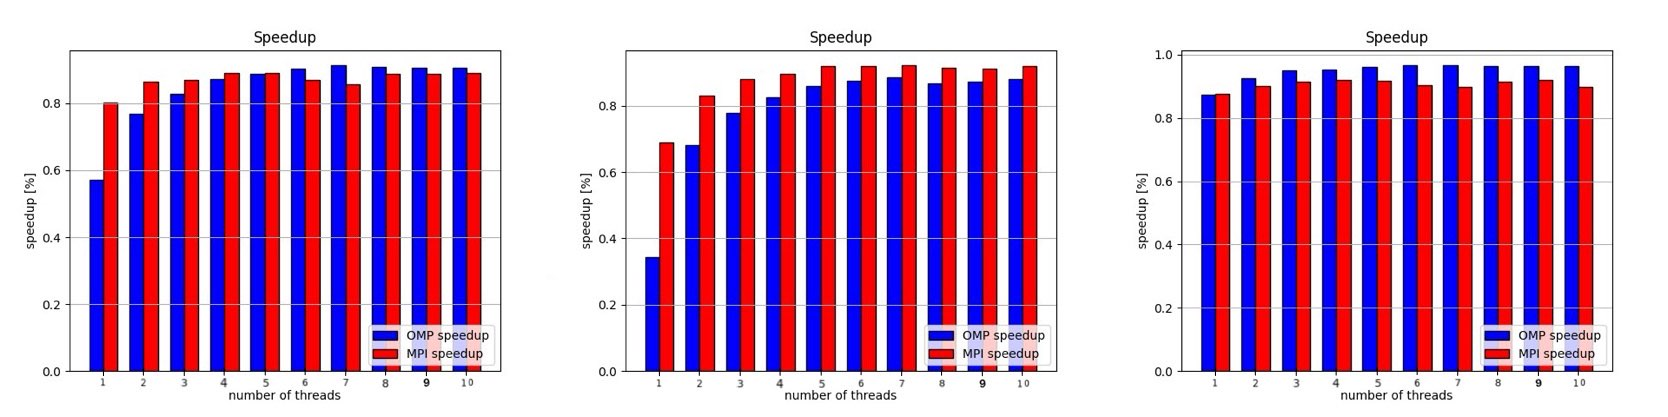
\includegraphics[width = 0.85\textwidth]{imgs/suhghpts.jpg}
\end{figure*}

\subsection{Large workloads}
Increasing the workload doesn't change the overall behavior of the parallel execution, i.e. both the OMP and the MPI improve by increasing the number of threads, with the MPI one being a little bit faster than the OMP version. This is true even for larger workload given that the number of points is not too high. In the latter case, the OMP version becomes faster than the MPI version and this happens because of process zero in the MPI version. 
Once it has gathered the updated critical points from the other processes it has to iterate through all of them to update the corresponding points in the points array. Therefore the more points, means the more criticals (particularly in the first phases). This doesn't happen if the number of centroids is high, because process zero can directly gather the updated centroids inside the centroids array, and neither does it occur for the dimension.

To show this behavior, Figure \ref{fig:suslow} shows three different situations: on the left there is the case of a random dataset with a complexity of (19020, 10, 2) in the center another random dataset with a complexity of (1902, 10, 20) and on the right a downloaded dataset\footnote{https://archive.ics.uci.edu/dataset/159/magic+gamma+telescope, high energy gamma particles in an atmospheric Cherenkov telescope} with the same dimension of the first one. In this case the total complexity is $19020\cdot 10\cdot 2 = 380400$ for all the cases which is almost twice the complexity of 200000 used for the previous testing.

It can be seen that, even if the total complexity of all the datasets is the same, when the number of points is high then the OMP version is slightly faster than the MPI version. But in the middle case when the number of points is lower then the behavior is the usual one with the MPI being faster than the OMP version.

\subsection{Conclusions}
In every case, the Hamerly algorithm is faster than the Lloyd version even with one thread. 

Increasing the number of threads improves the performace in every case if the complexity of the dataset is large enough.

Finally, increasing the complexity doesn't change the overall behavior (except for higher execution times) but if the number of points is too large than the OMP version runs faster than the MPI one, which is usually not the case for other combinations of N, K and D.

\section{Platform and computing system description}
All the tests were executed on a Windows 11 PC with an AMD Ryzen 7 5800H (3.20 GHz) processor and 16 GB of RAM. To run the MPI code has been used the Microsoft MPI library \cite{b2}.

\section{Future work}
This project can be further improved by implementing some enchangements.
In the MPI version, process zero has to do more work than the other processes because it has to manage all the other process by scattering and gathering all the total variables. This could be balanced by partitioning all the variables between the processes even if applying this method would require a more complex strategy to handle the criticals scattering.In addition, a more advanced version of the Hamerly's algorithm optimizes also the centroid repositiong as explained by a team of researchers from the North Carolina State University who introduced this optimization in their paper \cite{b3} .

\begin{thebibliography}{00}
  \bibitem{b1} Partitional Clustering Algorithms by M. Emre Celebi, \url{https://link.springer.com/chapter/$10.1007$/978-3-319-09259-1_2}, Chapter 2.
  \bibitem{b2} MSMPI, \url{https://www.microsoft.com/en-US/download/details.aspx?id=57467}
  \bibitem{b3} Yufei Ding, Yue Zhao, Xipeng Shen, Madanlal Musuvath,  and Todd Mytkowicz, ``Yinyang K-Means: A Drop-In Replacement of the Classic K-Means with Consistent Speedup''.
\end{thebibliography}

\end{document}